\documentclass[tikz,border=5pt]{standalone}
\usetikzlibrary{shapes.geometric, arrows}

\tikzstyle{process} = [rectangle, rounded corners,
minimum width=4cm, minimum height=1cm,
text centered, draw=black, fill=blue!15]

\tikzstyle{arrow} = [thick,->,>=stealth]

\begin{document}
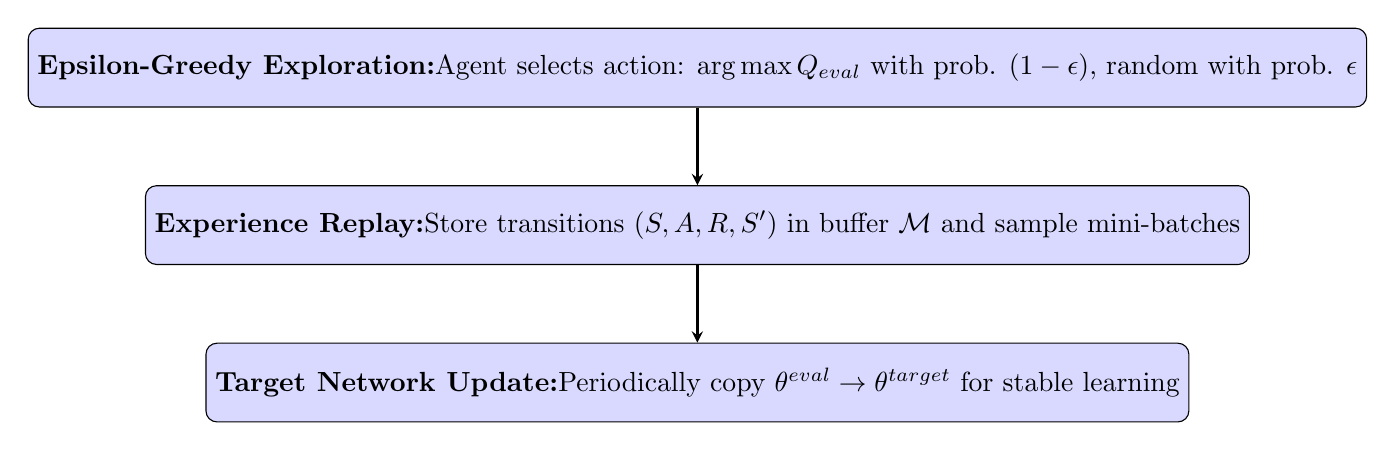
\begin{tikzpicture}[node distance=2cm]

% Nodes
\node[process] (exploration) {\textbf{Epsilon-Greedy Exploration:}\\
Agent selects action: $\arg\max Q_{eval}$ with prob. $(1-\epsilon)$, random with prob. $\epsilon$};

\node[process, below of=exploration] (replay) {\textbf{Experience Replay:}\\
Store transitions $(S,A,R,S')$ in buffer $\mathcal{M}$ and sample mini-batches};

\node[process, below of=replay] (target) {\textbf{Target Network Update:}\\
Periodically copy $\theta^{eval} \to \theta^{target}$ for stable learning};

% Arrows
\draw[arrow] (exploration) -- (replay);
\draw[arrow] (replay) -- (target);

\end{tikzpicture}
\end{document}
